\section{Розробка та тестування програмного забезпечення}
\subsection{Особливості програмної реалізації системи, що розробляється}
Для розробки програмної системи була використані мова програмування Kotlin та застосовані патерни проектування типу GoF та принципи SOLID та Сlean architecture.

SOLID --- це абревіатура складена з перших літер п'яти базових принципів об'єктно-орієнтованого програмування та дизайну запропонована Робертом Мартіном~\cite{Arch2007}:
\begin{enumerate}
	\item Принцип єдиного обов'язку --- принцип об'єктно-орієнтованого програмування, який означає, що клас має бути створений для виконання лише однієї задачі, яку він повинен повністю інкапсулювати. 
	Отже, всі сервіси цього класу мають бути повністю підпорядковані її виконанню. 
	Результатом слідування цій концепції є наявність лише однієї причини для зміни класу.
	\item Принцип відкритості/закритості --- принцип об'єктно-орієнтованого програмування, який означає, що програмні сутності, такі як класи, модулі, функції, методи та ін. мають бути <<відкритими для розширення та закритими для змін>>. 
	Це означає, що вони можуть надавати можливість змінювати свою поведінку без або з мінімальними змінами коду.
	\item Принцип заміщення Лісков --- якщо $S$ підтип $T$, тоді об'єкти типу $T$ в програмі можуть бути заміщені об'єктами типу $S$ без будь-яких змін бажаних властивостей цієї програми.
	\item Принцип розділення інтерфейсів --- принцип схожий із принципом єдиного обов'язку. 
	Застосування даного принципу полягає у розділі занадто <<товстих>> інтерфейсів на менші та специфічні, щоб їх клієнти знали лише про ті методи, що необхідні для них у роботі. 
	Як результат, при зміні певного функціоналу, незмінними мають лишитися ті класи, що не використовують його. 
	Тобто виконання цього принципу допомагає системі залишатися гнучкою при внесенні до неї змін та лишатися простою для рефакторингу.
	\item Принцип інверсії залежностей. 
	Принцип формулюється наступним чином: модулі вищого рівня не повинні залежати від модулів нижчого рівня, обидва типи модулів повинні залежати від абстракцій; абстракції не повинні залежати від деталей реалізації, деталі реалізації повинні залежати від абстракцій.
\end{enumerate}

Чиста архітектура полягає в розділенні системи на 3 рівні~\cite{Arch2007}: 
\begin{enumerate}
	\item Рівень даних --- рівень даних у чистому вигляді, що складається з сутностей, які є основними бізнес-правилами системи.
	\item Доменний рівень --- рівень бізнес-логіки додатку, що відповідає за основний функціонал системи, її поведінку та правила, що стосуються конкретного додатку.
	\item Рівень представлення --- рівень користувацького інтерфейсу, відображення даних, обробки користувацьких подій.
\end{enumerate}

\subsection{Тестування програмного забезпечення}
\subsubsection{Загальна теорія тестування}
Тестування --- перевірка відповідності реальної поведінки програми очікуваній, що здійснюється на кінцевому наборі тестів, який був обраний певним чином. 
У більш широкому сенсі, тестування --- це одна з технік контролю якості, що включає в себе активності з планування робіт, проектування тестів, виконання тестування і аналізу отриманих результатів.

Верифікація --- це процес оцінки системи або її компонентів з метою визначення чи задовольняють результати поточного етапу розробки умовам, що були сформовані на початку цього етапу. 
Тобто чи виконуються наші цілі, терміни, завдання по розробці проекту, визначені на початку поточної фази.

Валідація --- це визначення відповідності ПО, що розроблюється очікуванням і потребам користувача, вимогам до системи. 

\subsubsection{Порядок проведення тестування програмного забезпечення, що розроблюється}
На першому етапі тестування необхідно провести модульне тестування усіх компонентів системи, які можуть бути протестовані окремо від інших у штучному середовищі тестування. 
Unit-тестування буде проведено за допомогою засобу автоматизації тестування Junit.

Такий вибір зумовлений простотою інтеграції Junit з Kotlin. 
Junit надає великий об'єм валідаційних методів, завдяки яким можна легко та ефективно тестувати як модулі обробки даних та взаємодії з базами даних, так і модулі вводу та виводу інформації.

Приклад застосованих Junit тестів приведено нижче:
\begin{lstlisting}
var assert = require('assert');
describe('Basic mocha tests', function () {
 it('Array should contain min 4 elements', function () {
        assert.equal(ServerObject.data.length, 4);
    });
 it('should return type of object, function () {
        assert.equal(typeof ClientObject.data, typeof {});
    });
});

it('should return true if valid type', function(){
      var isValid = import.isValidTypeOfData(data);
      assert.equal(isValid, true);
});
it('should return false if invalid type', function(){
      var isValid = import.isValidTypeOfData('data');
      assert.equal(isValid, false);
});
\end{lstlisting}

У подальшому необхідно виконати інтеграційне тестування, що передбачає тестування у двох напрямках.
Інтеграційне тестування компонентного рівня після unit-тестування необхідне для перевірки правильної взаємодії частин бізнес-логіки додатку. 
Завдяки такому тестуванню можна виявити помилки реалізації зовнішніх інтерфейсів або ж їх некоректне використання.

Інтеграційне тестування системного рівня необхідне для знаходження можливих помилок у взаємодії різних підсистем програмного забезпечення, його взаємодії з операційною системою, іншими додатками.
На етапі системного тестування необхідно визначити, чи відповідає розроблена програмне забезпечення визначеним функціональним та нефункціональним вимогам.
Для цього необхідно виконати усі визначені сценарії використання в умовах, що близькі до реальних. 
Даний етап є дуже важливим, тому що існує ризик виявлення таких дефектів, як відсутність або неправильна реалізація функціональності, невиконання таких функціональних вимог, як зручність використання, захищеність, продуктивність тощо. 
На етапі системного тестування виконують остаточну перевірку сумісності програмного забезпечення та операційної системи.

Найвищим рівнем тестування є прийомне тестування, що виконується до тих пір, поки його результати не задовольнять замовника та інших зацікавлених осіб.

\subsection{Графічний інтерфейс програмного забезпечення}
На рисунку~\ref{fig:screenshot} зображено графічний інтерфейс прототипу програмного засобу для моделювання розподільчих логістичних систем.

\begin{figure}[H]
	\centering
	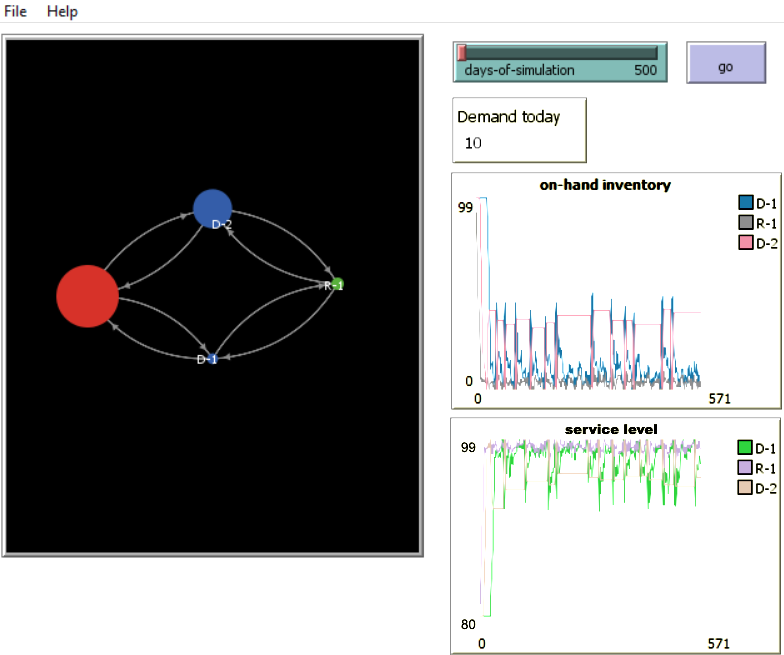
\includegraphics[width=\textwidth]{screenshot}
	\caption{Графічний інтерфейс програмного забезпечення}
	\label{fig:screenshot}
\end{figure} 

Графічний інтерфейс складається з двох частин: меню та панелі поточного стану моделі.

Меню складається з двох пунктів:
\begin{enumerate}[label={\arabic*)}]
	\item File --- пункт, з якого можна загрузити конфігурацію логістичної системи (рис.~\ref{fig:screenshot_open}) та зробити звіт (рис.~\ref{fig:screenshot_report});
	\item Help --- пункт, в якому міститься базова інформація о програмі та автору.
\end{enumerate} 

Панель поточного стану моделі складається з візуального представлення моделі (де \textit{D-1}, \textit{D-2} --- постачальники, \textit{R-1} --- роздрібний продавець, інше --- головний склад), кнопки запуску симуляції та графіків рівня запасу та рівня сервісу.

\begin{figure}[H]
	\centering
	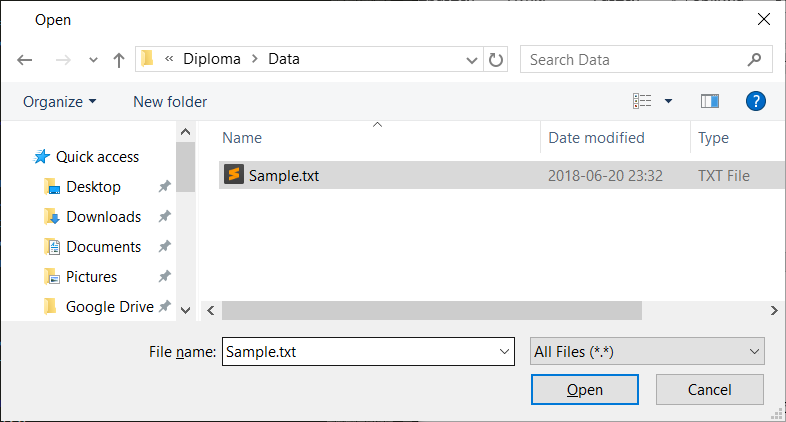
\includegraphics[width=0.6\textwidth]{screenshot_open}
	\caption{Діалог завантаження файлу конфігурації}
	\label{fig:screenshot_open}
\end{figure}

\begin{figure}[H]
	\centering
	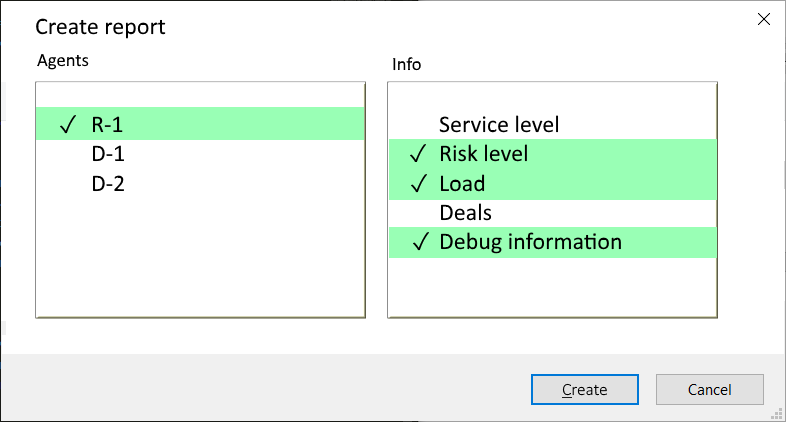
\includegraphics[width=0.6\textwidth]{screenshot_report}
	\caption{Діалог створення звіту}
	\label{fig:screenshot_report}
\end{figure} 

\subsection{Аналіз та шляхи вдосконалення системи}
Шляхом вдосконалення системи може бути розробка підтримки формату GIS для завантаження мапи та об'єктів з карти.

Іншим шляхом може бути перенос логіки програми на виділений сервер та розміщення клієнтної часті в мережі Інтернет.
Таким чином зменшиться порог доступу для користивання програмою, збільшиться рівень захищеності програми.
Мінусами такого рішення буде можливе зменшення швидкості роботи програми, необхідність підключення до мережі Інтернет.
